\documentclass[letterpaper,twocolumn,12pt]{article}
\usepackage{usenix2020_09}
\usepackage{amsmath}
\usepackage{url}
\usepackage{hyperref}
\usepackage{graphicx}
\usepackage{dblfloatfix}

\microtypecontext{spacing=nonfrench}

% define todo as a red text with [TODO: ]
\newcommand{\todo}[1]{\textcolor{red}{[TODO: #1]}}

\usepackage{tikz}
\usetikzlibrary{positioning, arrows.meta}

\begin{document}

\date{}
% \title{Hardware-Aware Scheduling for Microservices with On-Chip Accelerators\thanks{The project repository is available at \url{https://github.com/liam0215/anarres}.}}
% \title{Project Checkpoint}
% \title{Hardware-Aware Scheduling for Microservices with On-Chip Accelerators}
\title{Annares: Acceleration-Aware Hardware Allocation for Microservices\thanks{The project repository is available at \url{https://github.com/liam0215/anarres}.}}


\author{
{\rm Liam Arzola, Ye Shu}\\
University of California, San Diego
}

\maketitle

\section{Introduction}

\subsection{Motivation}

Data centers today pay a ``tax'' on workloads comprised of common operations that support running modern applications in the cloud.
In 2015, Google published a paper characterizing the problem of the ``datacenter tax,'' in which they profiled thousands of machines over a three-year period to find that nearly 30\% of all cycles in the fleet belonged to just a handful of low-level operations~\cite{kanev2015profiling}.
Instead of being spent on business logic, these cycles were spent on auxiliary tasks such as serialization, RPC management, memory allocation, and compression/decompression.
These operations are common across many services, and thus optimizing them can yield significant performance improvements across a wide range of applications.
This discovery, paired with the end of Dennard scaling and the subsequent slowdown in the improvement of single thread performance, led to a decade of increased interest in low latency ``on-chip'' accelerators, which are better suited for offloading small granularity datacenter tax operations.
For example, Intel's Sapphire Rapids CPUs introduced the Intel In-line Accelerator (IAA) for operations such as memory copy and fill, (de)compression, and de/encryption~\cite{yuan2024intel}.

Along with other forms of CPU heterogeneity, like the presence of energy-efficient cores and performance cores, the introduction of on-chip accelerators has led to increased complexity when choosing on which hardware to deploy an application.
For example, an application with insufficient instruction-level parallelism that is often stalled on accesses to memory may be better placed on efficiency cores; in contrast, an application with more instructions per cycle would be better off running on performance cores~\cite{kanev2015profiling}.

In this project, we aim to present a preliminary study on the trade-off between the cost of offloading operations to specialized accelerators and the overhead of migrating workloads between different hardware cores.

\subsection{Problem Statement}

Scheduling applications on heterogeneous hardware is not a new problem; it is a hot topic in machine learning research~\cite{narayanan2023hetero,subramanya2023sia}.
However, despite the growing heterogeneity of special purpose hardwares, general-purpose applications like microservices have not had as much attention, especially with regard to hardware heterogeneity.
Currently, if developers want to optimize the hardware allocation for their microservice, they have to manually profile it on different hardware platforms, potentially swapping out specialized libraries to take advantage of local accelerators.

Manual profiling also struggles to keep up with the dynamic nature of changing workloads in production.
For example, a microservice that is CPU-bound under one workload might become memory-bound under another, and thus would benefit from being migrated to a different hardware platform.
The lack of a feedback loop between runtime telemetry and scheduling decisions means that many potential performance are at best underutilized and at worst wasted.

In this project, we aim to address the problem of scheduling microservices on heterogeneous hardware by designing a system that continuously profiles the cost of operations within a microservice and informs real-time decisions on whether to offload these operations to specialized accelerators.

\subsection{Contributions}

We propose a system for automatically detecting when an operation within a microservice would benefit enough from offloading the operation to an on-chip accelerator to warrant migrating the microservice to different hardware.
The system makes the following contributions:

\begin{itemize}
    \item Microservice Telemetry.

    Microservices communicate profile statistics for different operations to a centralized scheduler service that makes an allocation decision.

    \item Telemetry-driven Centralized Scheduler.

    The scheduler service makes allocation decisions, reconfigures and recompiles the necessary microservices to run on the allocated new hardware, and redeploys the microservices.

    \item Blueprint Plugin for IAA Acceleration.

    We extend the blueprint microservice platform with a plugin that allows Go programs to invoke the Intel IAA for compression and decompression operations using native Intel IAA APIs.

    \item Microbenchmarking Framework \& Tradeoff Analysis.

    We build a suite of microbenchmarks to characterize network overhead versus accelerator invocation cost, giving insights into when offloading truly pays off.
\end{itemize}

With these pieces in place, our system closes the loop from telemetry to placement to execution, ensuring that microservices automatically exploit the full spectrum of compute resources available in modern servers.


\section{Design}
We propose a system for automatically detecting when an operation within a microservice would benefit enough from offloading the operation to an on-chip accelerator to warrant migrating the microservice to different hardware.
Microservices communicate profile statistics for different operations to a scheduler service that makes an allocation decision, reconfigures and recompiles the necessary microservices to run on the allocated new hardware, and redeploys the microservices.
We propose a simple centralized scheduler for collecting telemetry and making the allocation decision.


\section{Implementation}

Our final artifact will include the following:
\begin{itemize}
    \item The Blueprint workflow code for our compressed object cache microservice.
    \item The Blueprint plugin code to wrap Intel's QPL library for utilizing the IAA (or performing (de)compression in software if the IAA is not present).
    \item The Blueprint scaffolding code for the monolithic and microservice configurations.
    \item The benchmark code for orchestrating the experiments and measuring the end-to-end latency, system throughput, and CPU utilization for the different deployments.
    \item Telemetry code for monitoring (de)compression operation size.
    \item Scheduler code for polling telemetry information and choosing to reconfigure and redeploy the application.
\end{itemize}

\subsection{Project Progress}

We have made significant progress on the project so far.
We spent substantial time getting familiar with Blueprint and reading through example microservices, but are now making good progress on the implementation.
\begin{itemize}
    \item We have implemented all of the Blueprint workflow code except for the actual calls to the compression library.
    \item We are currently implementing the Blueprint plugin code to wrap Intel's QPL library by implementing a C shim layer and using Go's FFI to call the shim layer.
    \item We have implemented the scaffolding code for building the application as a single process or as separate Docker containers communicating over gRPC.
    \item We have yet to implement the code to run the experiments and collect measurements.
    \item We have yet to implement the telemetry code for monitoring (de)compression operation size.
    \item We have yet to implement the scheduler code for polling telemetry information and making allocation decisions.
\end{itemize}
For our evaluation, we will be running on two Intel Sapphire Rapids servers, one with the IAA enabled and one without.


\section{Results}
\begin{figure*}[!ht]            % “*”→span both columns; [!t]→force it to the top
  \centering
  % first image, take roughly half the page width:
  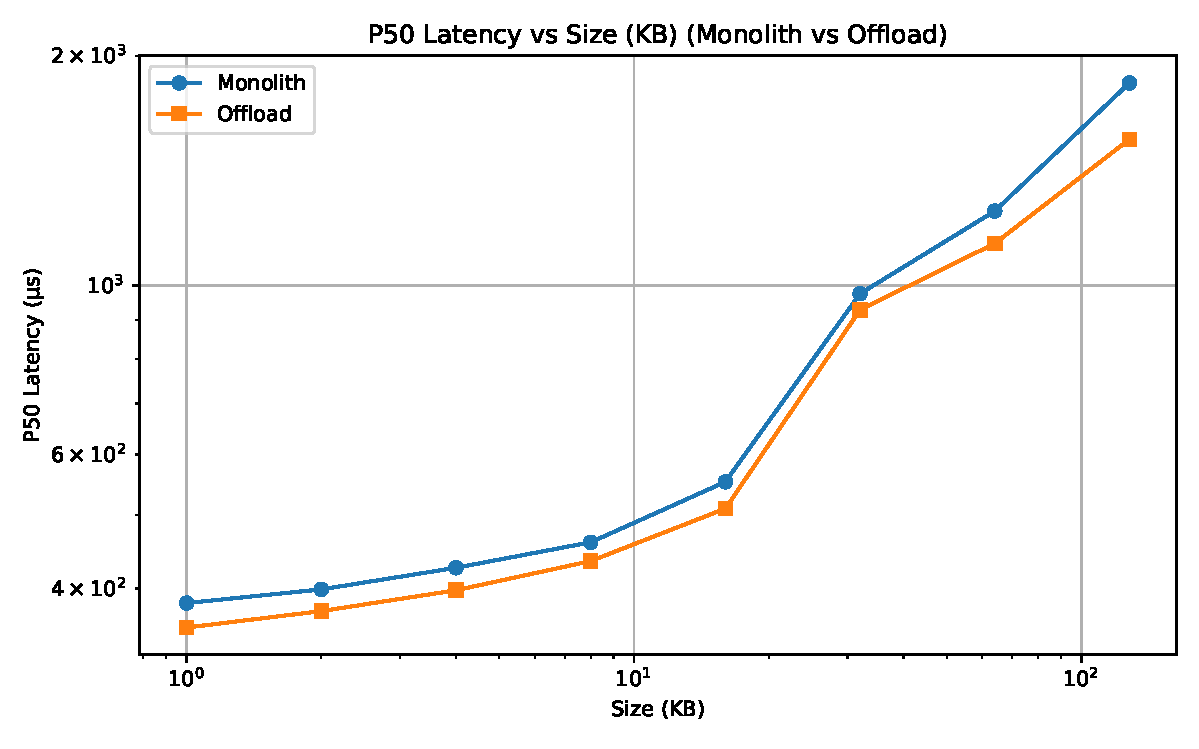
\includegraphics[width=0.48\textwidth]{size.pdf}%
  \hfill
  % second image:
  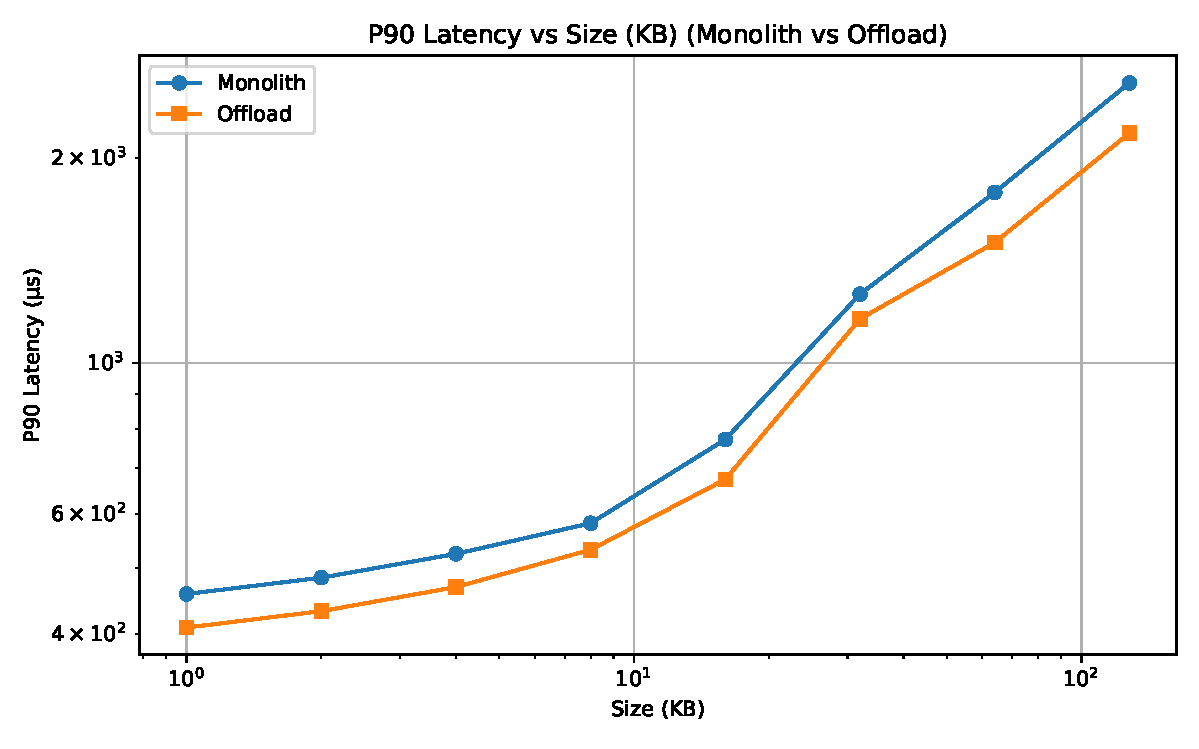
\includegraphics[width=0.48\textwidth]{size_p90.pdf}
  \caption{Median and 90th percentile latency versus the size of the input data. Sizes vary from 1KB to 128KB, with a data point at each power of two. Past 128KB, the latency increases by several orders of magnitude for both the monolithic configuration and the microservice (offload) configuration, so we omit those data points for clarity. The offered load is fixed at 4,000 requests per second. For both median and tail latency, the microservice configuration with offloaded (de)compression performs marginally better than the monolithic configuration.}
  \label{fig:size}
\end{figure*}

\begin{figure*}[!ht]            % “*”→span both columns; [!t]→force it to the top
  \centering
  % first image, take roughly half the page width:
  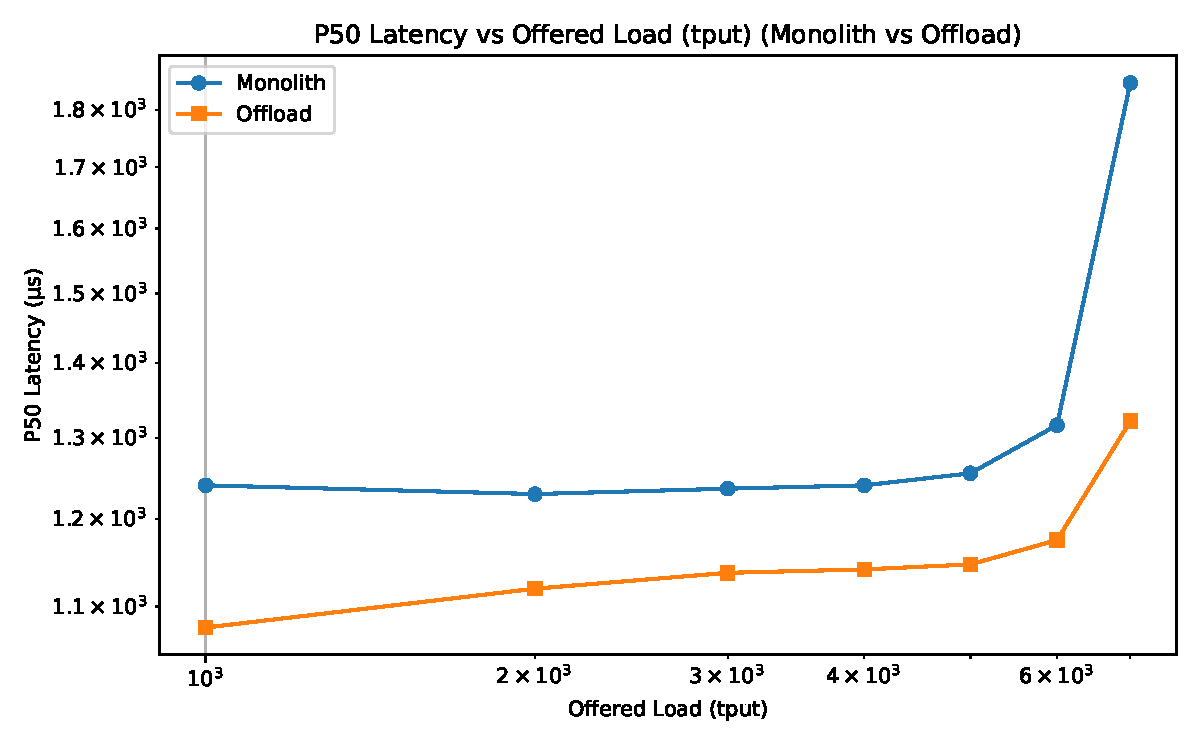
\includegraphics[width=0.48\textwidth]{p50.pdf}%
  \hfill
  % second image:
  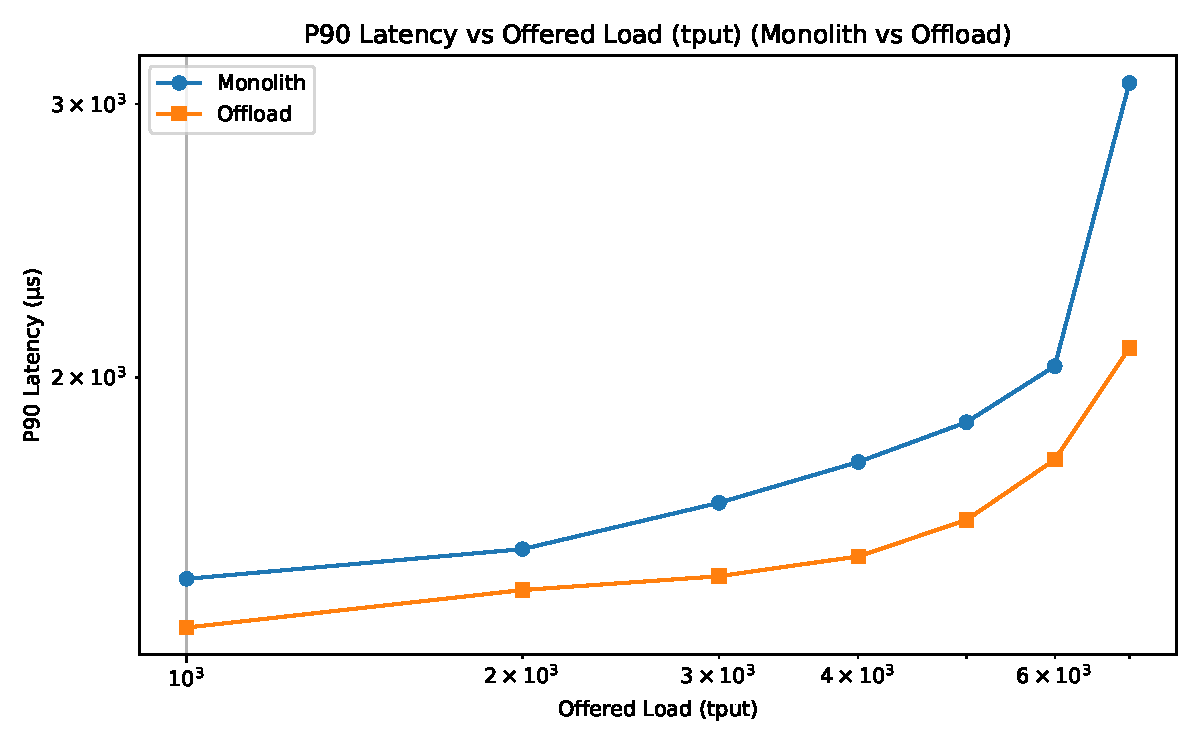
\includegraphics[width=0.48\textwidth]{p90.pdf}
  \caption{Median and 90th percentile latency versus the offered load. The load varies from 1,000 requests per second to 7,000. Past 7,000 requests per second, the latency increases by several orders of magnitude for both the monolithic configuration and the microservice (offload) configuration, so we omit those data points for clarity. The input data size is fixed at 64KB. Again, for both median and tail latency, the microservice configuration with offloaded (de)compression performs marginally better than the monolithic configuration.}
  \label{fig:tput}
\end{figure*}

\subsection{Experimental Setup}
We conduct experiments using one dual-socket server, each with a 28-core Intel Xeon Gold 5420+ CPU operating at 2.0 GHz and 256 GB of RAM. 
Hyperthreading was enabled. 
The operating system was Ubuntu 24.04. 
We pinned all containers to one socket, and we only used the IAA device local to the socket. 
The IAA was configured with 8 shared work queues and 8 engines.

\subsection{Service Configurations}
We evaluated two configurations for the compressed cache service.
\begin{enumerate}
  \item A monolithic configuration that places the frontend service and compression service in the same process and the same container. Communicating between the two services is done through a local function call. The QPL software path is used for (de)compression.
  \item A microservice configuration that splits the frontend service and compression service into separate containers, requiring that they communicate over gRPC, but offloading the (de)compression operations to the IAA.
\end{enumerate}
For both, we use Memcached as the cache implementation, which is hosted in its own container and accessed by the frontend service via gRPC. Likewise, the scheduler service is hosted in its own container and communicates with the compression service to collect operation metrics over gRPC.


\section{Related Works}

In this section, we first review the sources of the “datacenter tax,” then survey prior work on CPU heterogeneity and hardware-aware scheduling, and finally discuss existing approaches to offloading (de)compression in microservice and big-data frameworks.

\subsection{The Datacenter Tax}

The term ``datacenter tax'' refers to the overhead incurred by low-level operations that are common across data center workloads, which can consume a significant fraction of CPU cycles in production environments.
% In the Google 2015 paper \citetitle{kanev2015profiling}

In the 2015 paper \cite{kanev2015profiling} and a succeeding 2019 book \cite{barrosoDatacenterComputer2019} by Google, they discovered that a surprisingly large fraction of CPU time---up to ``one out three compute cycles at Google'' \cite[p. 165]{barrosoDatacenterComputer2019}---gets spent in just a handful of low-level, shared software routines rather than in application logic. They dub this overhead the ``datacenter tax'' and break it down into six components:

\begin{itemize}
    \item Protobuf management that serializes and deserializes data passed between RPC services.
    \item RPC libraries that perform load balancing, encryption, and failure detection.
    \item Further data movement with direct call of \texttt{memcpy} or \texttt{memmove}.
    \item General-purpose compression. Although the authors do not specify the exact scenarios, they specify that ``[a]pproximately one quarter of all tax cycles are spent compressing and decompressing data'' \cite[p. 162]{kanev2015profiling}.
    \item Memory allocation, specifically for recursive data structures.
    \item Hashing, which are mostly for cryptographic hash functions used during communication.
\end{itemize}

Because these routines are both small and common to many services, targeting them for hardware acceleration or microarchitectural optimization promises far higher payoff per engineering dollar than chasing hotspots in individual binaries.

In our project, we explore the optimization trade-off of the general-purpose compression and decompression operations, which are a significant part of the datacenter tax, using the Intel In-line Accelerator (IAA).

\subsection{Hardware-Aware Scheduling}

Modern CPUs expose heterogeneous types of compute resources to programmers, including:
\begin{itemize}
  \item \emph{Performance cores} (P-cores) that are high-performance and out-of-order,
  \item \emph{Efficiency cores} (E-cores) that are energy-efficient and in-order, and
  \item \emph{On-die accelerators} that are specialized for low-latency operations, such as Intel IAA for (de)compression.
\end{itemize}
These heterogeneous resources require new scheduling policies to maximize performance and energy efficiency.
This problem is not new; it has been studied in the context of both CPU and accelerator scheduling.

\subsubsection{Heterogeneous CPU Scheduling}

Early work by \cite{menasceStaticDynamic1995} proposes and compares static and dynamic processor assignment in a single-ISA heterogeneous parallel architecture.
They introduce dynamic feedback policies that allow jobs to migrate between fast and slow processors based on their execution characteristics, improving overall utilization, and thus throughput and response time.
However, their work relies on an idealized Markovian model of service times, and ignores the migration overheads and practical constraints of real-world systems.

Building on this, \cite{ghiasiSchedulingHeterogeneous2005} targets server and cluster systems whose cores share an ISA but differ in voltage/frequency capabilities.
They propose a run-time adaptive scheduler that monitors per-thread performance counters and dynamically map threads and reduce energy cost.

Similarly, \cite{topcuogluTaskScheduling1999} statically schedules workloads on heterogeneous processors using a DAG.
Their HEFT (Heterogeneous Earliest Finish Time) and CPOP (Critical Path On a Processor) heuristics rank tasks by critical paths using a DAG and assign them to cores statically.
However, the methodology requires an accurate a priori knowledge of task execution time, which may not be feasible in practice.
Also, the static nature of the scheduling may not adapt well to dynamic workload changes.

More recently, \cite{clarkProcessorAcceleration2003} proposes a fully automated framework using data flow graph.
A compiler-driven dataflow-graph exploration engine identifies critical subgraphs, which are then offloaded to custom functional units integrated into the core pipeline.
These instructions are then synthesized and accelerated while preserving ISA compatibility.
However, their alleged automation still requires manual intervention and incurs extra verification overhead for correctness.

Together, these works span a spectrum of scheduling strategies on historical heterogeneous CPUs, laying a comprehensive groundwork for modern heterogeneous hardware scheduling that also involves on-chip accelerators.

\subsubsection{Accelerator Scheduling}

Beyond CPU cores, on-chip accelerators introduce another dimension to scheduling.

Panneerselvam et al. \cite{panneerselvamOperatingSystems2012} argue for treating and scheduling accelerators as OS resources.
Their prototype integrates an accelerator monitor in the kernel to broker access, enforce QoS, and virtualize devices across processes.

Augonnet et al. \cite{augonnetDataAwareTask2010} extend accelerator with a data-aware scheduler that overlaps DMA transfers and kernel launches across multiple GPUs.
By prefetching data blocks as soon as dependencies are satisfied, they reduce accelerator idle time and boost throughput.
However, their scheme depends on accurate transfer-time models, which may not be feasible.

Gupta et al. \cite{guptaPegasusCoordinated2011} present Pegasus, which interposes in the Xen hypervisor to queue and dispatch accelerator access across VMs under global fairness and tail-latency objectives.

Huang et al. \cite{huangCoSAScheduling2021} introduce CoSA, which aims to reduce the exponential scheduling search space of DNN-specific spatial accelerators by formulating computation and data movements as a mixed-integer programming (MIP) problem.
CoSA outperforms heuristic scheduling tools while reducing scheduling time.

\subsection{Accelerator Offload for Microservices and Data Centers}

In practice, offloading work from CPUs to accelerators is beginning to find its way into microservice and data‐center workflows, but only in proof-of-concept settings.
Sriraman et al. introduce Accelerometer \cite{sriramanAccelerometerUnderstanding2020}, a predictive model that predicts realistic speedups when offloading common microservice building blocks at Facebook scale.
Similarly, Liu et al.'s E3 \cite{liuE3EnergyEfficient2019} extends Azure Service Fabric to offload whole microservices onto SmartNICs, demonstrating energy savings and performance improvements.

Beyond these proofs of concept, there is a significant gap: no general-purpose scheduler seamlessly coordinates CPUs, GPUs, FPGAs, and SmartNICs across microservice workloads at data-center scale, leaving operators without unified policies for dynamic offload across diverse accelerator classes.

Our work bridges these domains by combining fine-grained telemetry, centralized decision logic, and potential for migration using Kubernetes to automate the offload of (de)compression to hardware accelerators in microservice environments.


\section{Conclusion}

some takeaways


\bibliographystyle{plain}
\bibliography{references}

\end{document}
